% !TeX encoding = UTF-8
% !TeX spellcheck = de_DE
% !TeX program = lualatex
% !BIB program = biber

\documentclass[ngerman, aspectratio=169]{beamer}
\usepackage{polyglossia} \setdefaultlanguage{german}

\usepackage{fontspec} \setsansfont{Noto Sans} \setmonofont{Noto Mono}
\usepackage{unicode-math}

\usepackage{multicol}

\usepackage[sorting=none]{biblatex}
\addbibresource{literature.bib}

\usetheme{frisbeesportverband}

\title{Ernährung im Ultimate}
\date{\today}
\author[M. Brandt]{Matthias Brandt}
\institute{Deutscher\par Frisbeesport-Verband e.V.}

\begin{document}
\begin{frame}
  \titlepage
\end{frame}

\begin{frame}
  \frametitle{Übersicht}
  \tableofcontents
\end{frame}

\section{Grundlagen}
\begin{frame}
  \frametitle{Vorweg}
  \begin{columns}
    \begin{column}{0.7\textwidth}
      \begin{itemize}
        \begin{itemize}
        \item Erkenntnisse aus Sport- und Ernährungswissenschaften ändern sich ständig
        \item Heute Goldstandard, morgen Quatsch
        \item Unter Umständen vereinfacht dargestellt
        \item Quelle, falls nicht anders angegeben:\\ \textcite{raschka2015sport}
        \end{itemize}

      \end{itemize}
    \end{column}
    
    \begin{column}{0.3\textwidth}
      \begin{figure}
        \centering
        \includegraphics[width=\textwidth, height=0.8\textheight, keepaspectratio]{images/iceberg.png}      
        \caption{Nach \cite{kils2005iceberg}}
        \label{fig:iceberg}
      \end{figure}
    \end{column}
    
  \end{columns}
\end{frame}


\begin{frame}
  \frametitle{Nährstoffe}
  \begin{multicols}{2}
    \begin{itemize}
      
    \item<+-> Hauptnährstoffe
      \begin{itemize}
      \item Kohlenhydrate
      \item Protein
      \item Fett
      \item Alkohol
      \item Ballaststoffe
      \end{itemize}
      
    \item<+-> Wasser
      
      \vfill\null
      \columnbreak
      
    \item<+-> Mikronährstoffe
      \begin{itemize}
      \item Fettlösliche Vitamine (E, D, K, A)
      \item Wasserlösliche Vitamine (B, C)
      \end{itemize}
      
    \item<+-> Mineralstoffe
      \begin{itemize}
      \item Mengenelemente (Elektrolyte)
      \item Spurenelemente
      \item Ultraspurenelemente
      \item Sekundäre Pflanzenstoffe
      \end{itemize}

    \end{itemize}
    
  \end{multicols}
  
\end{frame}

\section{Kohlenhydrate}
\begin{frame}
  \frametitle{Übersicht}
  \begin{itemize}
  \item Kohlenhydrate sind wichtigster Energielieferant
    \begin{itemize}
    \item Stellen Energie schnell zur Verfügung
    \item Emfehlung: 60\% der Energiezufuhr aus Kohlenhydraten
    \end{itemize}

  \item Sportler nehmen oft zu wenige Kohlenhydrate auf
  \end{itemize}
\end{frame}

\begin{frame}
  \frametitle{Auswahl}
  \begin{multicols}{2}
  \begin{itemize}
  \item<+-> Grundbaustein: Monosaccharide (Einfachzucker)
    \begin{itemize}
    \item Glucose, Fructose (Früchte, Honig, kleine Mengen in Pflanzen)
    \end{itemize}
  \item<+-> Zwei- und Mehrfachzucker:
    \begin{itemize}
    \item<+-> Disaccharide
      \begin{itemize}
      \item Saccharose (Zuckerrübe, Zuckerrohr, Früchte)
      \item Lactose (Milch und Milchprodukte)
      \item Maltose (Abbauprodukt von Stärke)
      \end{itemize}
      
      \vfill\null
      \columnbreak
    \item<+-> Oligosaccharide (3-10 Einfachzucker)
      \begin{itemize}
      \item Raffinose (Zuckerrübenmelasse, Honig, Hülsenfrüchte)
      \end{itemize}
    \item<+-> Polysaccharide (>10 Einfachzucker)
      \begin{itemize}
      \item pflanzliche Stärke (Stärke, Getreide, Kartoffeln)
      \item tierische Stärke (Artischoken, Chicorée, Zwiebeln, Spargel, Bananen)
      \end{itemize}
    \item<+-> Künstliche Zucker
      \begin{itemize}
      \item Dextrose
      \item Glukosesirup
      \end{itemize}

    \end{itemize}

  \end{itemize}
\end{multicols}
\end{frame}

\begin{frame}[allowframebreaks]
  \frametitle{Glykämischer Index}
  \begin{itemize}
  \item Reaktion des Blutzuckerspiegels auf ein Lebensmittel
  \item Hoher GI $→$ Höherer Blutzuckerspiegel
  \item Höherer Blutzuckerspiegel $→$ Größere Insulinantwort
  \item Größere Insulinantwort $→$ Schnellere Energieabgabe
  \item Beispiele
    \begin{itemize}
    \item Glukose - 100
    \item Weißes Baguette - 95
    \item Banane - 58
    \end{itemize}

  \end{itemize}
\framebreak
  \begin{columns}
    \begin{column}{0.7\textwidth}
      Aber

      \begin{itemize}
      \item Blutzuckerspiegel bei Sportlern steigt langsamer
      \item GI von Mahlzeiten schwer abschätzbar
      \end{itemize}
      
    \end{column}
    
    \begin{column}{0.3\textwidth}
      \begin{figure}
        \centering
        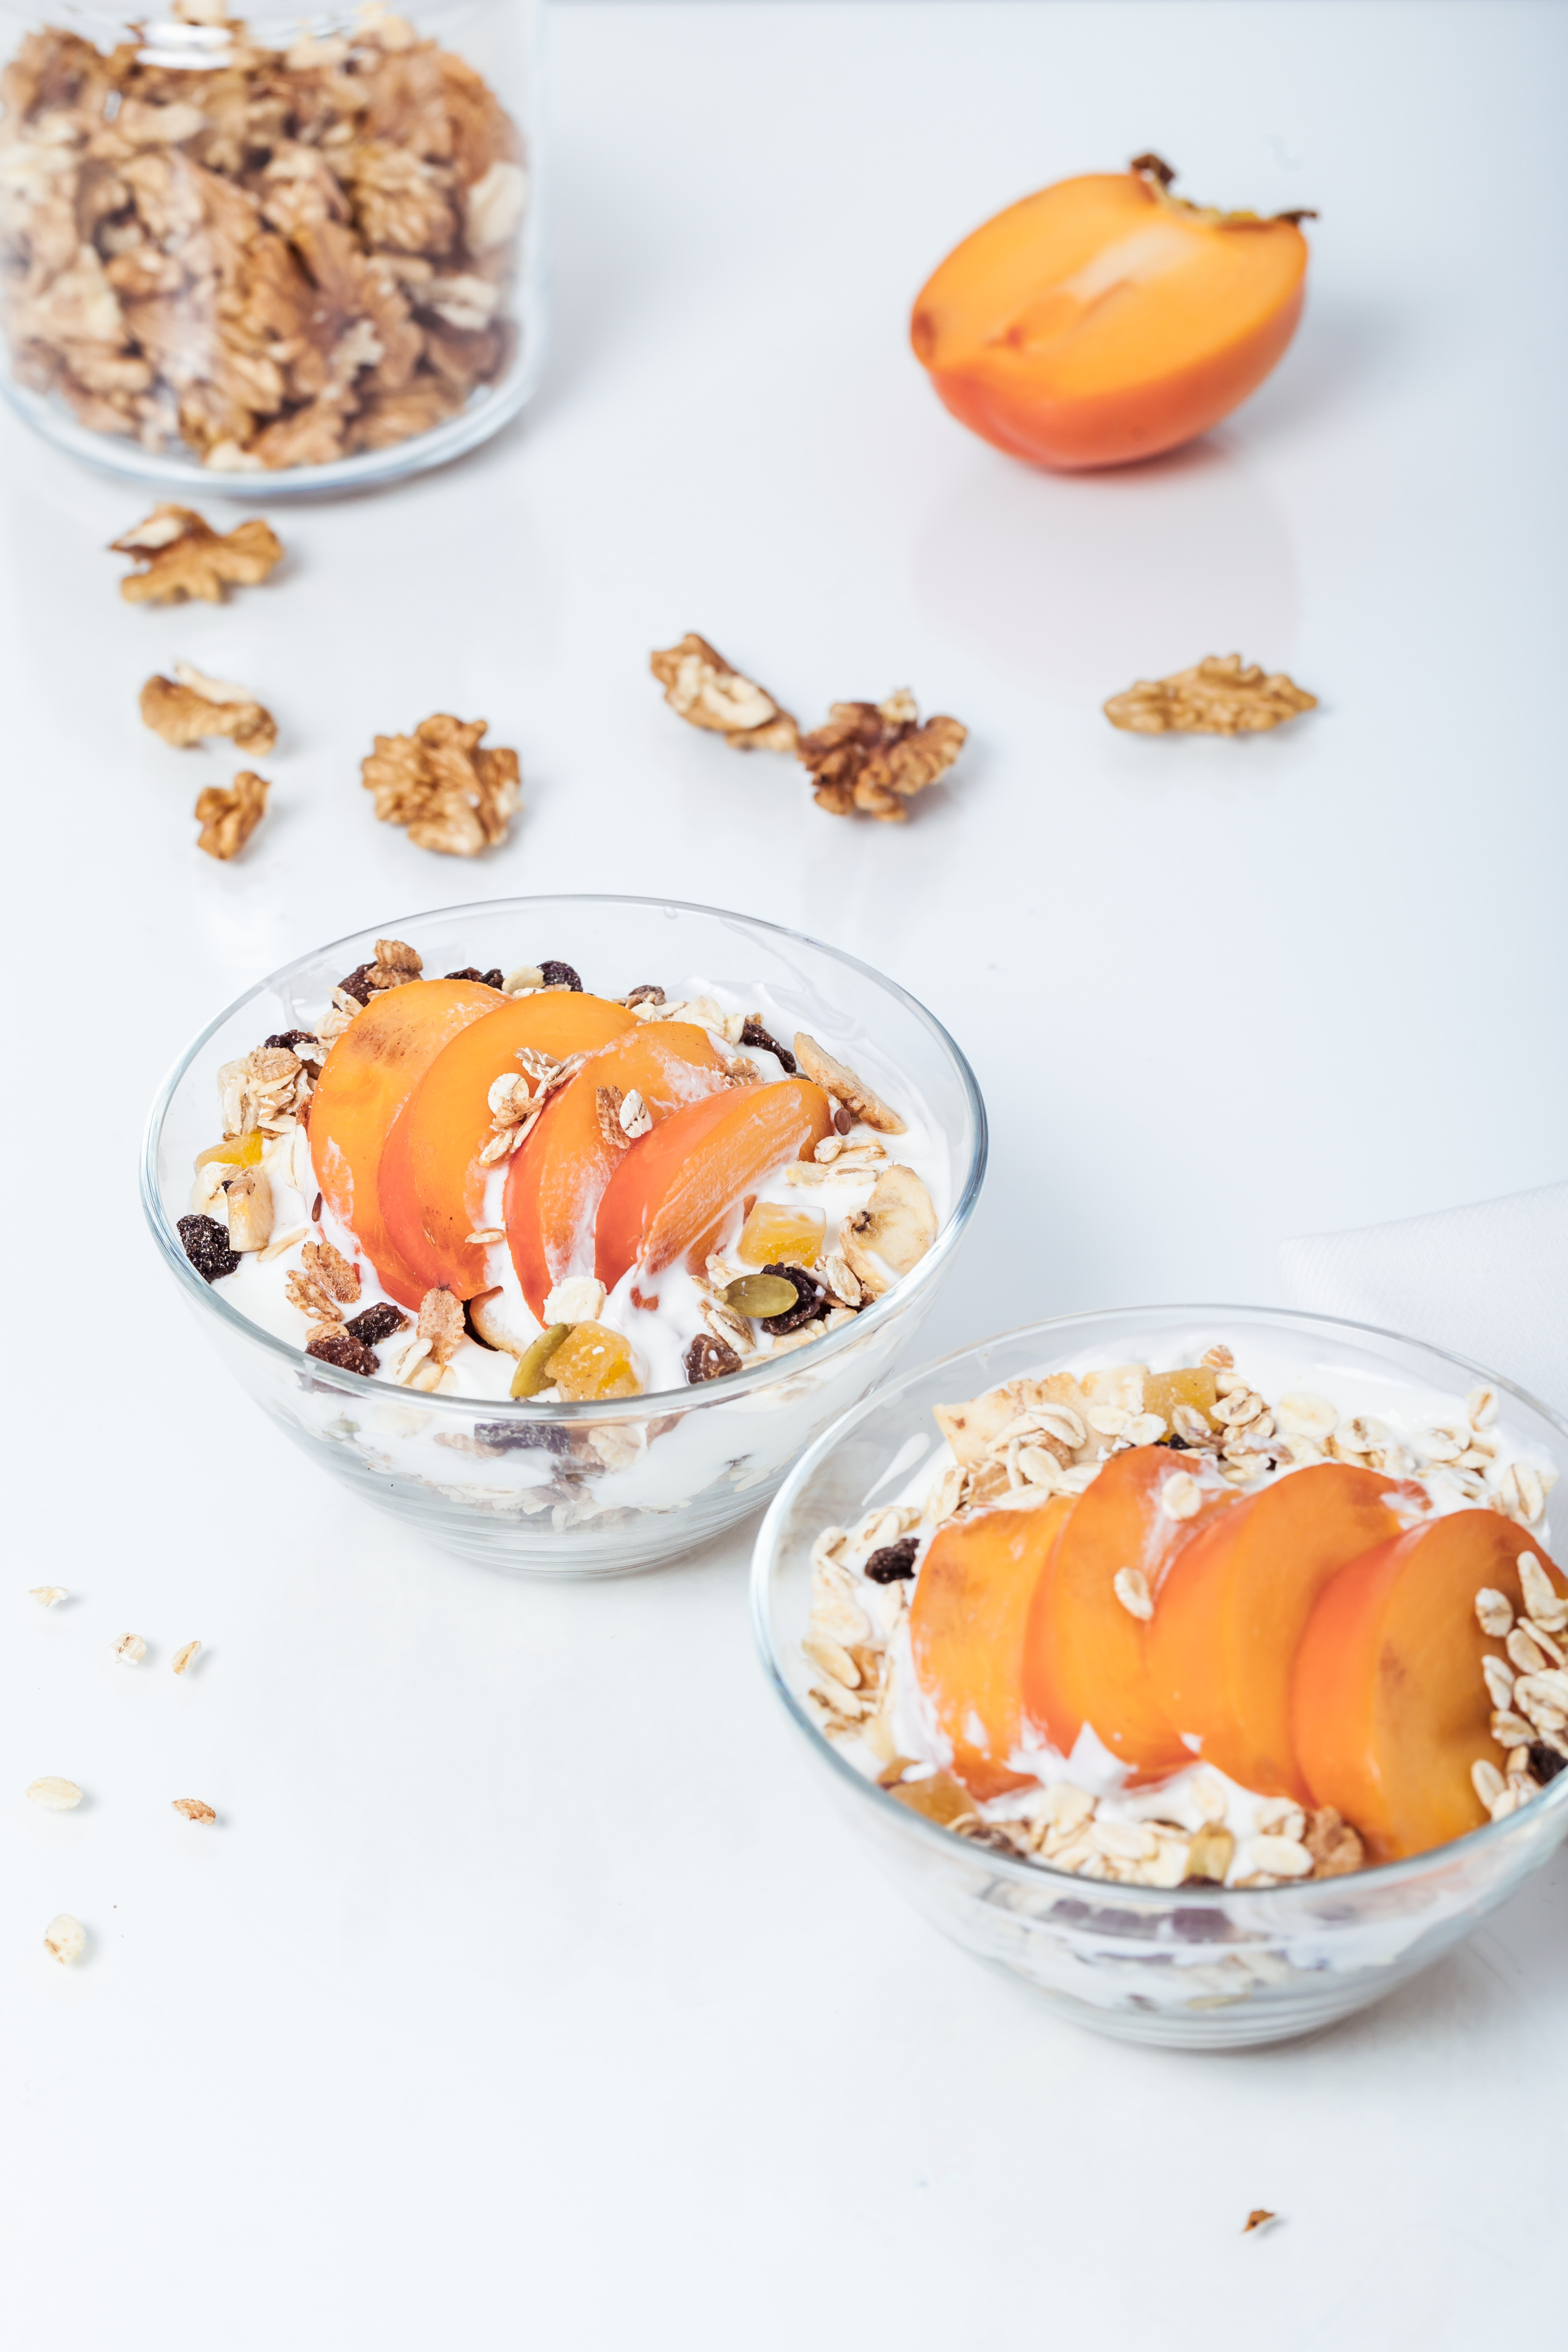
\includegraphics[width=\textwidth, height=0.8\textheight, keepaspectratio]{images/alexander-mils-372238-unsplash.jpg}      
        \caption{Müsli \cite{mills2017vegan}}
        \label{fig:breakfast}
      \end{figure}
    \end{column}
  \end{columns}

  \framebreak

  Vereinfacht

  \begin{itemize}
  \item Hoher GI für schnellen Energiebedarf (hyperglykämische Lebensmittel)
    \begin{itemize}
    \item Während des Sports oder bei kurzen Regenerationsphasen
    \item Hohe Aufnahme von Glucose und Saccharose vermeiden
    \item Stark verarbeitete Lebensmittel und Süßes
    \end{itemize}

  \item Niedriger GI für normalen Energiebedarf (hypoglykämische Lebensmittel)
    \begin{itemize}
    \item Vor der Belastung
    \item Unverarbeitete Lebensmittel, Vollkornprodukte
    \end{itemize}

  \item Kombination aus beidem für lange Wettkampftage

  \end{itemize}
  
\end{frame}

\section{Fette}
\begin{frame}
  \frametitle{Übersicht}
  \begin{itemize}
  \item<+-> Energielieferant (empfohlen \~{} 30\% der Energiezufuhr)
  \item<+-> Gute Energiedichte, aber langsame Freisetzung
  \item<+-> Vitamin„lieferant“ (fettlösliche Vitamine)
  \item<+-> Ungesättigte Fettsäuren (Flüssige Fette)
    \begin{itemize}
    \item Besonders Pflanzenöle
    \item Einfach ungesättigte Fettsäuren (10-13\% der Energiezufuhr)
    \item Mehrfach ungesättigte Fettsäuren (7-10\% der Energiezufuhr)
    \end{itemize}

  \item<+-> Gesättigte Fettsäuren (Feste fette) (10\% der Energiezufuhr)
    \begin{itemize}
    \item Besonders tierische Fette, Schokolade
    \item Haben viel Cholesterin (wird nur in geringen Mengen benötigt)
    \end{itemize}

  \end{itemize}
\end{frame}
\begin{frame}
  \frametitle{Tipps}
  \begin{columns}
    \begin{column}{0.7\textwidth}
      \begin{itemize}
      \item<+-> Aufnahme gesättigter Fette reduzieren
        \begin{itemize}
        \item „versteckt“ in Wurst, Chips, Sahne, fettem Käse, Gebäck und Schokolade
        \end{itemize}
      \item<+-> Pflanzliche Fette bevorzugen (z.B. zum Anbraten, zum Salat)
      \item<+-> Magere tierische Produkte
        \begin{itemize}
        \item Mageres Fleisch, Hartkäse, Magerquark, Hüttenkäse
        \end{itemize}
      \item<+-> Auf trans-Fettsäuren verzichten (enstehen bei Fetthärtung von Ölen)
      \item<+-> Fisch statt Fleisch

      \end{itemize}
    \end{column}
    
    \begin{column}{0.3\textwidth}
      \begin{figure}
        \centering
        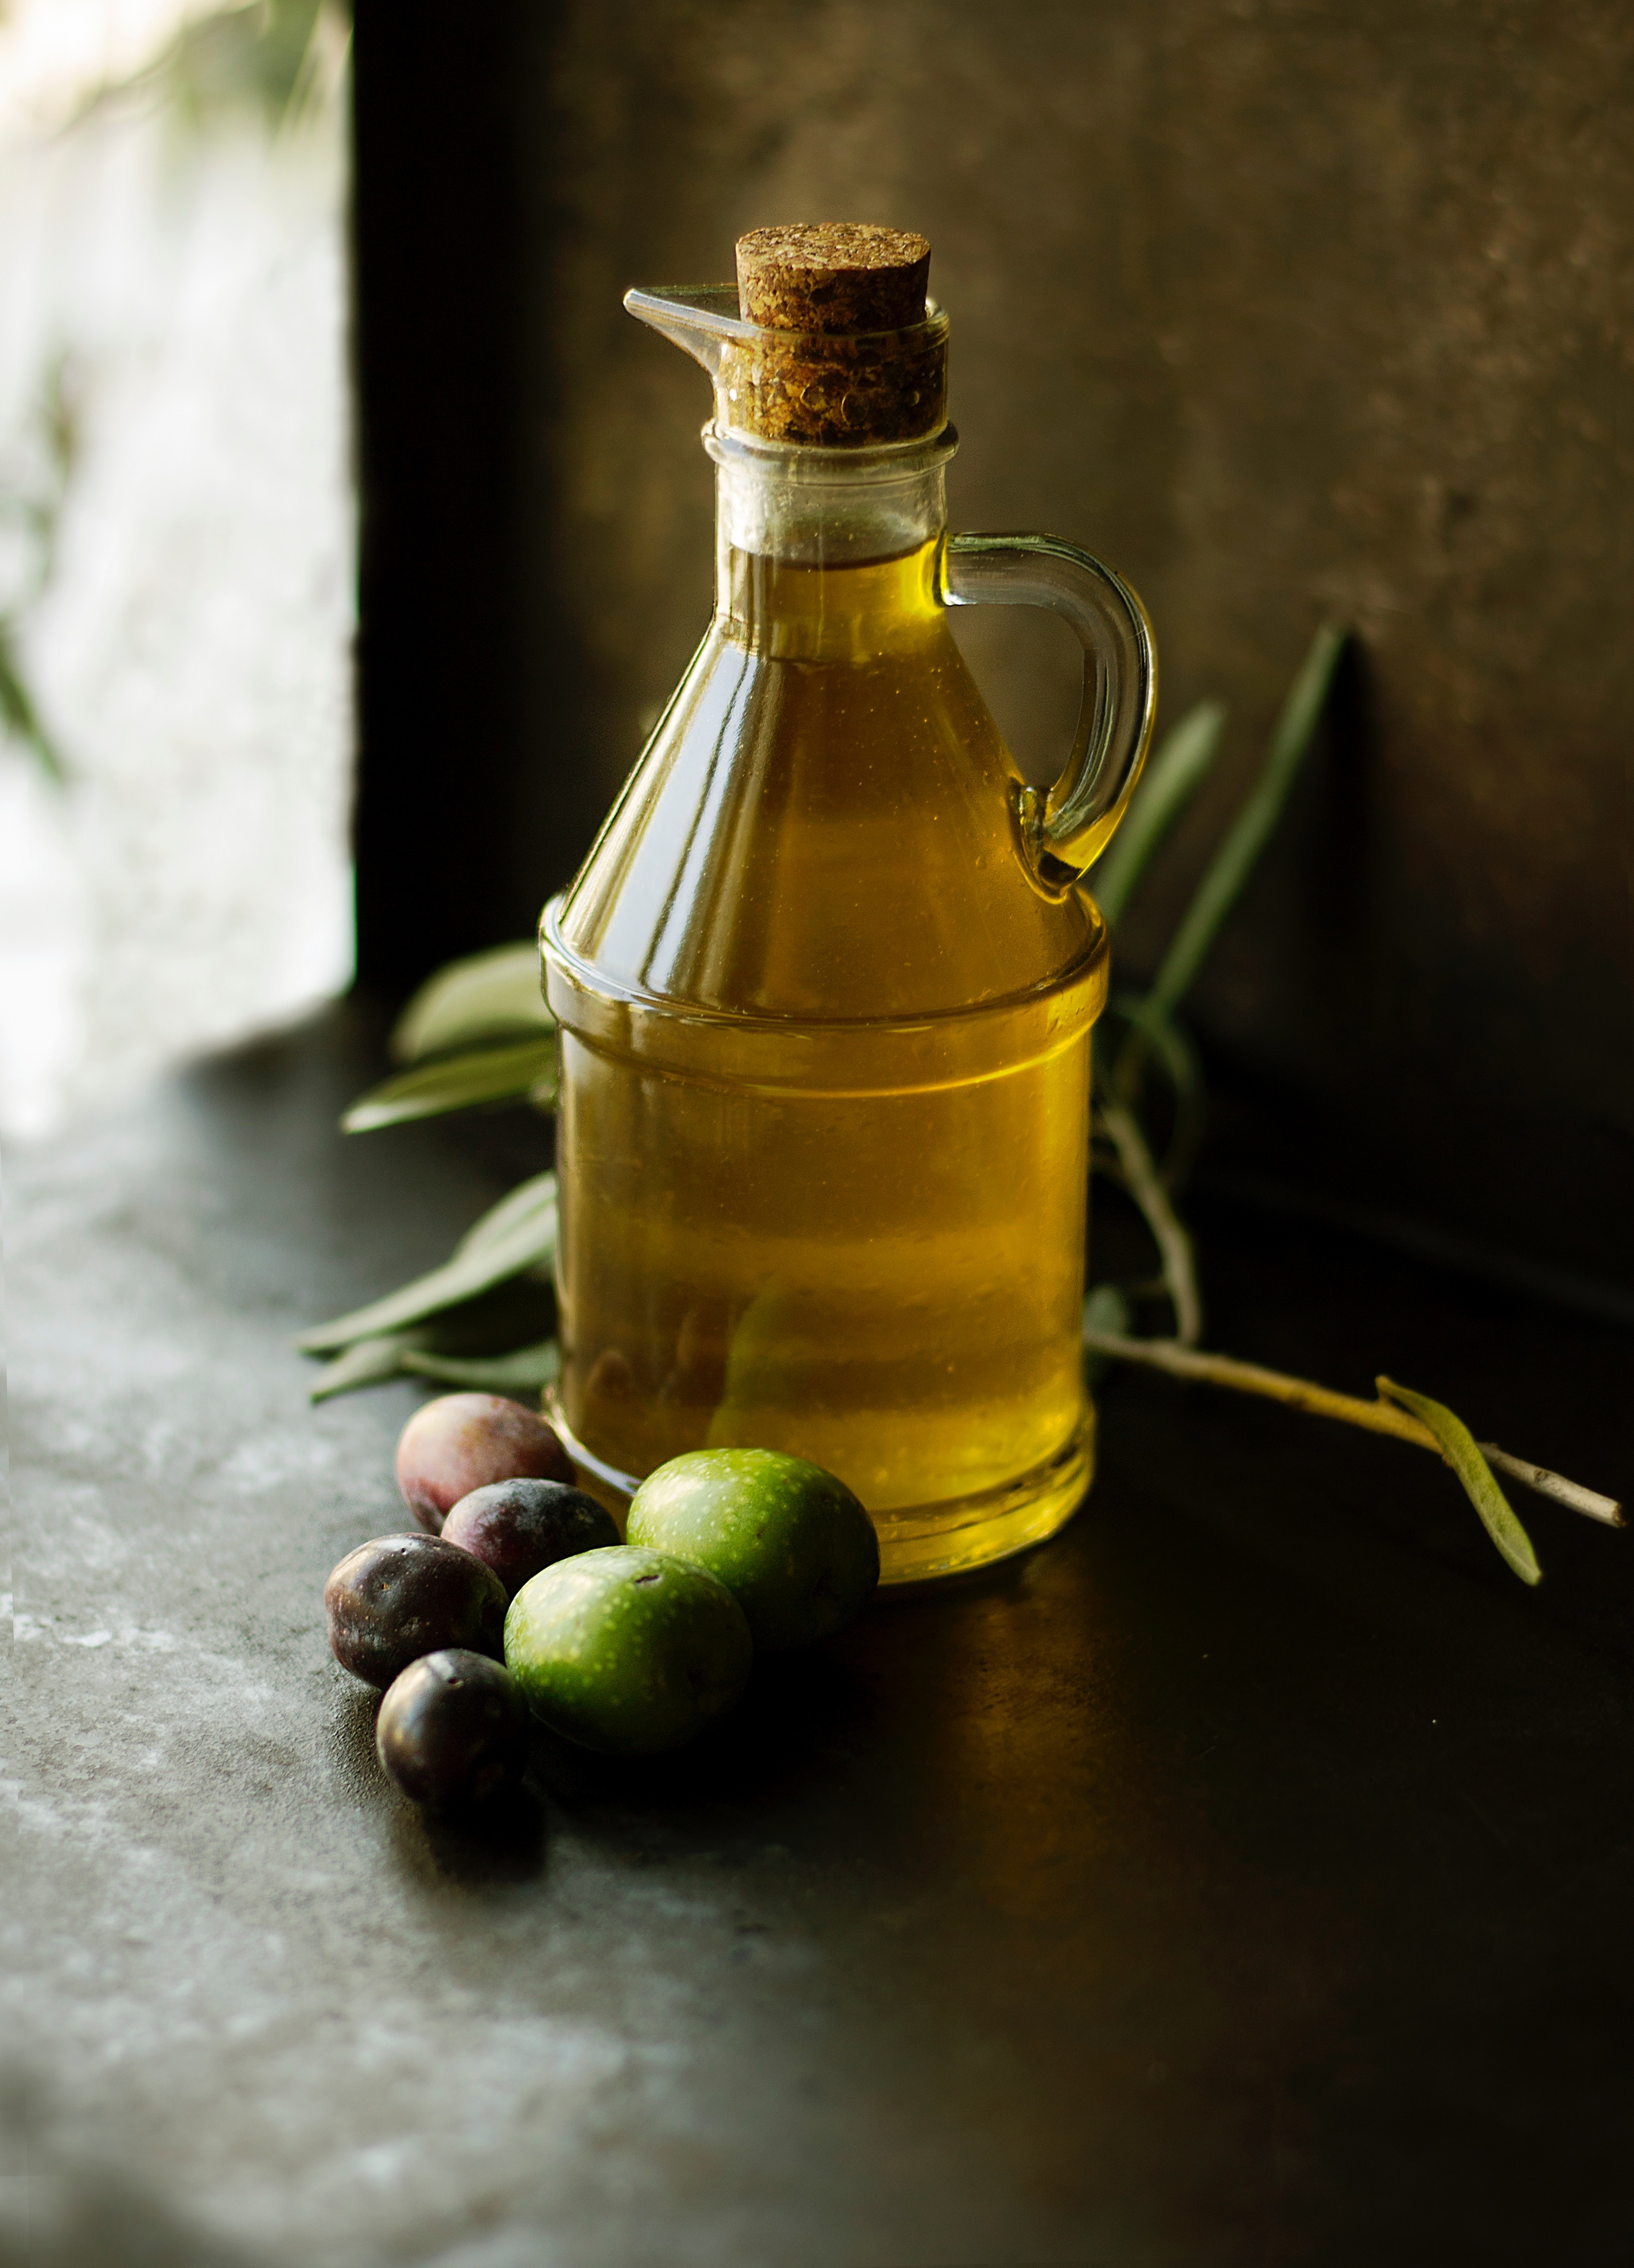
\includegraphics[width=\textwidth, height=0.8\textheight, keepaspectratio]{images/roberta-sorge-142255-unsplash.jpg}      
        \caption{Olivenöl \cite{sorge2016oil}}
        \label{fig:olvive-oil}
      \end{figure}
    \end{column}
    
  \end{columns}
\end{frame}


\section{Proteine}
\begin{frame}
  \frametitle{Übersicht}
  \begin{itemize}
  \item<+-> Ketten von Aminosäuren unterschiedlicher Länge
  \item<+-> Etwa 20 verschiedene Aminosäuren $→$ viele verschiedene Proteine
  \item<+-> Erfüllen Vielzahl von Funktionen
    \begin{itemize}
    \item Hormone, Enzyme, Antikörper
    \item Bindegewebe, Haut, Haare, Muskelfasern
    \end{itemize}
  \item<+-> Größter Speicher: Muskeln (\~{} 60\%)
  \item<+-> Wichtiger Baustoff für Muskeln
  \item<+-> Gute Eiweißquellen:\\ Milch- und Milchprodukte, mageres Fleisch, Fisch, Eier, Hülsenfrüchte
  \item<+-> Bedarf für Ausdauersportler: 1,2-1,4 g/kg (Frauen \~{} 10-20\% weniger)
  \item<+-> 12-15\% der Gesamtenergieaufnahme

  \end{itemize}

  
\end{frame}
\begin{frame}
  \frametitle{Proteinqualität}
  \begin{columns}
    \begin{column}{0.4\textwidth}

      \begin{itemize}
      \item<+-> Biologische Wertigkeit, Referenz: Eiprotein
      \item<+-> Körper kann Proteine höherer Qualität besser verarbeiten
      \item<+-> Kombinieren von Proteinen mit pflanzlichen Proteinen
      \item<+-> Qualität statt Quantität
      \end{itemize}
    \end{column}
    
    \begin{column}{0.6\textwidth}
      \visible<+->{
      \begin{figure}
        \centering
        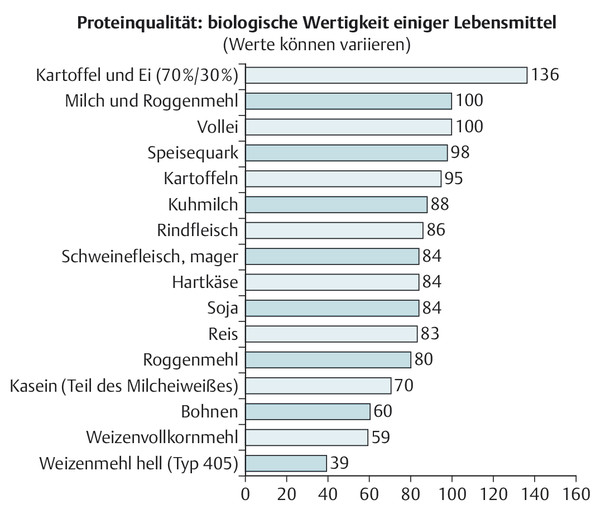
\includegraphics[width=\textwidth, height=0.8\textheight, keepaspectratio]{images/protein-quality.png}      
        \caption{Proteinqualität}
        \label{fig:proteine-quality}
      \end{figure}}
    \end{column}
    
  \end{columns}
\end{frame}


\section{Sonstiges}
\section{Nahrungsergänzungsmittel}


\section{Quellen}
\begin{frame}
  \frametitle{Quellen}
  \printbibliography
  

\end{frame}


\end{document}
